%
% Dokumentation
%

% Allgemeine Dokumenteigenschaften
\documentclass[a4paper,			% Druck auf DIN A4-Papier.
numbers=enddot,					% Die Kapitel bekommen einen Punkt.
chapterprefix=false,			% Das Wort "Kapitel:" wird gelöscht.
12pt,							% 12pt ist die Normalschriftgröße, weitere Möglichkeitenn sind 10pt oder 11pt.
pointlessnumbers				% Nummerierungen in den Kapiteln haben keinen finalen Punkt zb 1.1 statt 1.1.
]							
{scrreprt}  					% Dokumentart.

\setkomafont{chapter}{\Large}
\setkomafont{section}{\large}

% Präambel: Parameter die sich auf das Gesamte Dokument auswirken.
\usepackage{geometry}
\usepackage{float}
\usepackage[ngerman]{babel}				% "Neue" Deutsche Rechtschreibung
\usepackage{textcomp}					% Aktiviert das Eurosymbol. (Im Text schreiben mit \texteuro)
\usepackage[utf8]{inputenc}				% Direkte Eingabe von Umlauten im Text. (Dieser Code läuft nicht überall)
\usepackage{graphicx}					% Ermöglicht das anzeigen von Bildern
%\usepackage{babelbib}					% Für verschiedene Deutsche Stile des Literaturverzeichnis
\usepackage{apacite}
%\usepackage[babel, german=guillemets]{csquotes}
\usepackage[babel,german=quotes]{csquotes}
\usepackage{amsmath,amssymb}			% Das Mathe Paket "American Mathematic Society" laden
\usepackage[printonlyused]{acronym}		% Paket für das Abkürzungsverzeichnis
\usepackage{fancyhdr}					% Fancyhdr zum Nutzen von Kopf und Fußzeilen mit voreingestellten Formatierungen
\usepackage{xcolor}						% Verschiedene Farben sind direkt als white usw nutzbar
\usepackage{epstopdf}					% eps Postscript Dateien können direkt eingefügt werden
\usepackage{tocstyle}					% Das Inhaltsverzeichnis lässt sich konfigurieren
\usepackage{listings}					% Ermöglicht das Einfügen von Quellcode mit Kommentarhighlighting und Nummerierung aussen
\usepackage{subfig}						% 2 Bilder nebeneinander
\usepackage{chngcntr}
\usepackage{tabularx}
\usepackage{url}
\usepackage{alltt}

\counterwithout{figure}{chapter} 

\definecolor{dkgreen}{rgb}{0,0.6,0}
\definecolor{gray}{rgb}{0.5,0.5,0.5}
\definecolor{mauve}{rgb}{0.58,0,0.82}

\lstset{
  frame=top,frame=bottom,
  basicstyle=\small\normalfont\sffamily,    % the size of the fonts that are used for the code
  stepnumber=1,                           % the step between two line-numbers. If it is 1 each line will be numbered
  numbersep=10pt,                         % how far the line-numbers are from the code
  tabsize=2,                              % tab size in blank spaces
  extendedchars=true,                     %
  breaklines=true,                        % sets automatic line breaking
  captionpos=t,                           % sets the caption-position to top
  mathescape=true,
  stringstyle=\color{white}\ttfamily, % Farbe der String
  showspaces=false,           % Leerzeichen anzeigen ?
  showtabs=false,             % Tabs anzeigen ?
  xleftmargin=17pt,
  framexleftmargin=17pt,
  framexrightmargin=17pt,
  framexbottommargin=5pt,
  framextopmargin=5pt,
  showstringspaces=false      % Leerzeichen in Strings anzeigen ?
 }

\DeclareCaptionFormat{listing}{\rule{\dimexpr\textwidth+17pt\relax}{0.4pt}\par\vskip1pt#1#2#3}
\captionsetup[lstlisting]{format=listing,singlelinecheck=false, margin=0pt, font={sf},labelsep=space,labelfont=bf}






% Kapitel, Bilder, Abkürzungen usw werden zu Links, ohne roten Rahmen. DAS FUNKTIONIERT NICHT MIT APACITE!!!!
%\usepackage[plainpages=false,
%pageanchor=false,
%linkbordercolor=white,					% Die Rahmen werden weiß und sind somit nicht mehr im PDF sichtbar
%pdfpagelabels]
%{hyperref}								% Inhaltsverzeichnis wird als Lesezeichen im Adobe Reader angezeigt	

% Absatz-Einstellungen
\geometry{a4paper,
left=20mm,
right=20mm,
top=2.5cm,
bottom=2.5cm}
\parindent0ex							% Oberster Satz eines Absatzes wird NICHT eingerückt!
\parskip1.4ex plus0.2ex minus0.2ex


% Kopf und Fußzeile einbinden und festlegen.
\pagestyle{fancy}									% Eigenen Seitenstil verwenden
\fancyhf{} 											% clear all header and footer fields
\renewcommand{\headrulewidth}{1pt}					% Die Dicke der Kopfzeilen-Trennline wird auf 1pt festgelegt
\renewcommand{\footrulewidth}{1pt}					% Die Dicke der Fusszeilen-Trennline wird auf 1pt festgelegt
\fancypagestyle{plain}{}
\fancyhead[R]{}										% Kopfzeile Rechts
\fancyfoot[R]{\thepage}								% Fusszeile Rechts

% Inhaltsverzeichnis anpassen.
\usetocstyle{allwithdot}				% Fällt den Leerraum mit Punkten auf
\setcounter{tocdepth}{1}

% Das eigentliche Dokument.
\begin{document}

% Dokumentenweite Einstellungen und Kommandos
\nonfrenchspacing
\newcommand{\FigRef}[1]{Abbildung \ref{#1} auf Seite \pageref{#1}}
\newcommand{\TabRef}[1]{Tabelle \ref{#1} auf Seite \pageref{#1}}
\renewcommand*{\chapterheadstartvskip}{\vspace*{0pt}}					% Abstand vor Kapitelnamen
\renewcommand*{\chapterheadendvskip}{\vspace{1cm}}						% Abstand nach Kapitelnamen
\setlength{\headheight}{30pt}											% Höhe der Kopfzeile festlegen
\setlength{\footskip}{30pt}												% Abstand von Text zu Fusszeile festlegen

% Titelseite
%
% Dokumentation
%

% 1. Seite
\thispagestyle{empty}

\begin{figure}
\flushright						% rechtsbündig

\includegraphics[width=5cm,clip=]{Bilder/HHN_ab_40_mm_4c_pos4}\\
\end{figure}

\vspace*{1.0cm}

\begin{center}
{\Huge Benutzerdokumentation\\
\vspace{0.1cm} 
für die Software\\
\vspace{0.1cm} 
\textbf{we}Factor}

\vspace{3.0cm}

	{\Large Als Projektarbeit für die Vorlesung\\
\vspace{0.1cm}
	Labor für Softwareentwicklung und Project Skills\\
\vspace{0.1cm}
	im Studiengang Software Engineering\\
\vspace{0.1cm}
	der Hochschule Heilbronn\\

}
\end{center}

\vspace*{4.5cm}





Autor:\\
{\Large
Florian Wohlgemuth\\

 }
\vspace{1,5cm}
Heilbronn, \today
%\textbf{FIRMA}, Str. 1, 12345 Ort\\
%Betreuer: Dr. Jemand\\

\fancyhf{} 											% clear all header and footer fields
\renewcommand{\headrulewidth}{1pt}					% Die Dicke der Kopfzeilen-Trennline wird auf 1pt festgelegt
\renewcommand{\footrulewidth}{1pt}					% Die Dicke der Fusszeilen-Trennline wird auf 1pt festgelegt
\fancypagestyle{plain}{}
\fancyhead[R]{}										% Kopfzeile Rechts
\fancyfoot[R]{\thepage}								% Fusszeile Rechts

\pagenumbering{Roman}  								% Die Verzeichnisse werden entsprechend mit römischen Seitenzahlen beschriftet

% +++++++++++++++++++++++++++++++++++++ab hier beginnen (vor dem inhaltsverzeichnis)

% Aenderungshistorie
\begin{tabularx}{\textwidth}{|l|X|l|l|} \hline
       \textbf{Version}  	& \textbf{Name}   	& \textbf{Kapitel}  & \textbf{Datum}\\ \hline
       0.1           		& Florens Hückstädt & Kapitel 1 		& 31.12.20014\\
        \hline
\end{tabularx}

% Inhaltsverzeichnis
%
% Dokumentation
%

% Kapitel dem Inhaltsverzeichnis hinzufügen
\addcontentsline{toc}{chapter}{Inhaltsverzeichnis}			% 1. Argument {toc} = Table Of Contents
															% 2. Argument {chapter} = Ebene bestimmen!
															% 3. Argument {Name} = Name des Eintrags
\noindent

\tableofcontents
	\thispagestyle{plain}
	\newpage				% Neue Seite erzwingen

% Abkürzungsverzeichnis
%
% Dokumentation
%

% Kapitel dem Inhaltsverzeichnis hinzufügen
\addcontentsline{toc}{chapter}{Abkürzungsverzeichnis}			% 1. Argument {toc} = Table Of Contents
																% 2. Argument {chapter} = Ebene bestimmen!
																% 3. Argument {Name} = Name des Eintrags
\noindent

\thispagestyle{plain}

\chapter*{Abkürzungsverzeichnis}
\begin{acronym}[PP]
\acro{JRE}{Java Runtime Environment}



\end{acronym}


% Abbildungsverzeichnis
%
% Dokumentation
%

% Kapitel dem Inhaltsverzeichnis hinzufügen
\addcontentsline{toc}{chapter}{Abbildungsverzeichnis}			% 1. Argument {toc} = Table Of Contents
																% 2. Argument {chapter} = Ebene bestimmen!
																% 3. Argument {Name} = Name des Eintrags
\noindent

\thispagestyle{plain}


\listoffigures



\pagenumbering{arabic}  							% Der folgende Text wird mit arabischen Zahlen beschriftet



\include{Verwendete_Technologien}

\thispagestyle{plain}

\chapter{Installationsanleitung}\label{c_installationsanleitung}
Lorem ipsum dolor sit amet, consetetur sadipscing elitr, sed diam nonumy eirmod tempor invidunt ut labore et dolore magna aliquyam erat, sed diam voluptua. At vero eos et accusam et justo duo dolores et ea rebum. Stet clita kasd gubergren, no sea takimata sanctus est Lorem ipsum dolor sit amet. Lorem ipsum dolor sit amet, consetetur sadipscing elitr, sed diam nonumy eirmod tempor invidunt ut labore et dolore magna aliquyam erat, sed diam voluptua. At vero eos et accusam et justo duo dolores et ea rebum. Stet clita kasd gubergren, no sea takimata sanctus est Lorem ipsum dolor sit amet.


\section{Erforderliche Hard- und Software}\label{s_erforderliche_hw_sw}
Zum Betreiben der Anwendung ist ein \ac{JRE} bzw zum Entwickeln ein \ac{JDK} in der Version 8 erforderlich.
Dafür gelten folgende Systemvoraussetzungen laut \cite{oraclejsv}

\begin{description}
   \item[Windows]~\par
   \begin{itemize}

    \item Windows 8 (Desktop)
    \item Windows 7
    \item Windows Vista SP2
    \item Windows Server 2008 R2 SP1 (64-Bit)
    \item Windows Server 2012 (64 Bit)
    \item RAM: 128 MB
    \item Datenträgerkapazität: 124 MB für JRE; 2 MB für Java Update
    \item Prozessor: Mindestens Pentium 2 266 MHz-Prozessor
    \item Browser: Internet Explorer 9 und höher, Firefox, Chrome
   \end{itemize}
   
      \item[Mac OS X]~\par
      \begin{itemize}
    \item Intel-basierter Mac unter Mac OS X 10.8.3+, 10.9+
    \item Administratorberechtigungen für die Installation
    \item 64-Bit-Browser
      \end{itemize}
      
      Ein 64-Bit-Browser (Beispiele: Safari, Firefox oder Chrome) ist zur Ausführung von Oracle Java auf Mac OS X erforderlich.
      
   \item[Linux]~\par
   \begin{itemize}

    \item Oracle Linux 5.5+1
    \item Oracle Linux 6.x (32-Bit), 6.x (64-Bit)2
    \item Oracle Linux 7.x (64-Bit)2
    \item Red Hat Enterprise Linux 5.5+1, 6.x (32-Bit), 6.x (64-Bit)2
    \item Ubuntu Linux 12.04 LTS, 13.x
    \item Suse Linux Enterprise Server 10 SP2+, 11.x
    \item Browser: Firefox

   \end{itemize}
      
   
\end{description}

\section{Starten des Servers}\label{s_startserver}
Das Starten des Servers kann grundsätzlich über einen direkten java-Aufruf geschehen (siehe \ref{s_startserver_java}). Eine weitere Möglichkeit ist der Start des Servers über das Application-Plugin von gradle (siehe \ref{s_startserver_gradle}). Im Auslieferungszustand wird eine interne HSQLDB-Datenbank verwendet. Daher ist ein direktes Starten des Servers möglich. Zur Verwendung einer anderen Datenbank siehe Abschnitt \ref{s_config_db}.

\subsection{Starten des Servers über die Kommandozeile}\label{s_startserver_java}
Zum Starten des Servers über einen direkten Java-Aufruf mit der Kommandozeile sind folgende Schritte durchzuführen:
   \begin{enumerate}

    \item Navigation mit der Kommandozeile in das Root-Verzeichnis von weFactor und Ausführen folgenden Befehls:
    \begin{lstlisting}
    gradlew assemble
    \end{lstlisting}
    Dadurch wird im Verzeichnis /build/libs die Datei wefactor.jar erzeugt. Gradle ist im Projekt integriert und muss nicht separat installiert werden (siehe \ref{s_gradle}).
    \item Ausführen des jars über den Befehl:
    \begin{lstlisting}
    java -jar wefactor.jar
    \end{lstlisting}

   \end{enumerate}


\subsection{Starten des Servers über Gradle}\label{s_startserver_gradle}
Das Gradle Application-Plugin erweitert die Sprachen-Plugins um allgemeine anwendungsbezogene Tasks. Es erlaubt das Ausführen und Bündeln von Anwendungen für die \ac{JVM}.

Für weitere Informationen zur Verwendung von Gradle innerhalb des weFactor-Projeks siehe \ref{s_gradle}.

Für weitere Informationen zum Application-Plugin siehe
Gradle Dokumentation
\footnote{\url{http://www.gradle.org/docs/current/userguide/application_plugin.html}}.

\subsubsection{Gradle run}
Zum Starten des Servers über den Gradle-Task run sind folgende Schritte durchzuführen:
   \begin{enumerate}

    \item Navigation mit der Kommandozeile in das Root-Verzeichnis von weFactor
    \item Ausführen des Gradle-Befehls:
    \begin{lstlisting}
    gradlew run
    \end{lstlisting}

   \end{enumerate}

\subsubsection{Gradle distZip}
Der Task distZip erzeugt ein Distributionsarchiv mit den erforderlichen Bibliotheken und entsprechenden Startskripten. Zur Erzeugung der Distribution sind folgende Schritte notwendig:

   \begin{enumerate}

    \item Navigation mit der Kommandozeile in das Root-Verzeichnis von weFactor und Ausführen folgenden Befehls:
    \begin{lstlisting}
    gradlew distZip
    \end{lstlisting}
    Dadurch wird im Verzeichnis /build/distributions die Datei wefactor.zip erzeugt.
    \item Entpacken des zip-Archivs.
    \item Starten der Anwendung über das Startskript
        \begin{lstlisting}
        wefactor.bat
        \end{lstlisting}
        Das Startscript ist im bin-Verzeichnis zu finden.
        

   \end{enumerate}





\thispagestyle{plain}

\chapter{Konfiguration der Anwendung}\label{c_config}
Die Konfiguration der Anwendung findet hauptsächlich über die \emph{application.properties} Datei statt. Hier können sämtliche Werte wie zum Beispiel Datenbank-URL, Logging-Einstellung usw. festgelegt werden. Die Konfigurationsdateien befinden sich im Verzeichnis \emph{resources}. Siehe Listing \ref{lst:appprops} als Beispiel.

   \begin{lstlisting}[caption={application.properties},label={lst:appprops},language=Java]
app.name=weFactor

# IDENTITY (ContextIdApplicationContextInitializer)
spring.application.name=weFactor

logging.level.org.springframework.web: DEBUG
logging.level.org.hibernate: ERROR

# THYMELEAF (ThymeleafAutoConfiguration)
spring.thymeleaf.encoding=UTF-8
spring.thymeleaf.content-type=text/html


# EMBEDDED SERVER CONFIGURATION (ServerProperties)
server.tomcat.uri-encoding = UTF-8

spring.mvc.locale=en_UK
spring.mvc.date-format= dd/MM/yyyy

# INTERNATIONALIZATION (MessageSourceAutoConfiguration)
spring.messages.basename=messages
spring.messages.cacheSeconds=-1
spring.messages.encoding=UTF-8

    
   \end{lstlisting}
   Eine ausführliche Liste der Einstellmöglichkeiten ist in der Spring Dokumentation\footnote{\url{http://docs.spring.io/spring-boot/docs/current/reference/html/common-application-properties.html}} zu finden.
   
   
\section{Environments}\label{s_env}
Als Ergänzung zur \emph{application.properties} Datei können umgebungsspezifische Einstellungen festgelegt werden. Dafür muss folgende Namenskonvention eingehalten werden: \emph{application-{profile}.properties}.

So lassen sich zum unterschiedliche Datenbank-Einstellungen für die verschiedenen Zielumgebungen festlegen. Möchte man spezielle Properties für ein Profil mit dem Namen \emph{dev} anlegen. So haben sich diese in einer Datei mit dem Namen \emph{application-dev.properties} zu befinden. Profile können nun zum Beispiel über die VM-Arguments aktiviert werden (siehe Abbildung \ref{fig:active-profile}).
\begin{figure}[H]
    \centering
    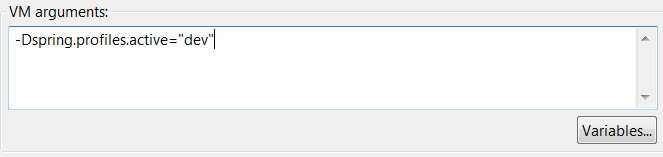
\includegraphics[width=0.8\textwidth]{Bilder/startlauncher.png}
    \caption{Profil über die VM-Arguments aktivieren}
    \label{fig:active-profile}
\end{figure}

\section{Konfiguration der Datenbank}\label{s_config_db}

\section{Konfiguration der Social-Login-Provider}\label{s_config_social}

\thispagestyle{plain}

\chapter{Entwicklung mit Eclipse}\label{c_eclipse}
In diesem Kapitel werden die Schritte beschrieben, die notwendig sind den Quellcode in Eclipse zu bearbeiten und die Anwendung darüber zu starten. Die Anleitung liegt zwar ausschließlich für Eclipse vor, es kann jedoch auch ein alternatives \ac{IDE} verwendet werden.
\section{Initialisierung und Import des Projekts}\label{s_initEclipse}
Zur Initialisierung des Projekts für Eclipse wird das Gradle-Plugin eclipse verwendet. Folgende Schritte sind durchzuführen:
   \begin{enumerate}

    \item Navigation mit der Kommandozeile in das Root-Verzeichnis von weFactor und Ausführen folgenden Befehls:
    \begin{lstlisting}
    gradlew eclipse
    \end{lstlisting}
    Dadurch werden folgende Dateien erstellt:
    \begin{itemize}
	    \item .project
	    \item .classpath
    \end{itemize}
    Außerdem werden alle notwendigen Bibliotheken von Gradle aus dem Internet geladen.
    \item Import des Projeks in Eclipse
       \begin{enumerate}
       	\item Über File/Import/Existing Project into Workspace Import-Dialog aufrufen.
       	\item Über die Schaltfläche Browse neben der Auswahlliste zu Selcet Root Directory das Wurzelverzeichnis des weFactor-Projekts auswählen.
       	\item Bestätigen über die Schaltfläche Finish.
       \end{enumerate}

   \end{enumerate}
   \section{Starten der Anwendung}\label{s_startFromEclipse}
   asdfsd





% Literaturverzeichnis
%
% Dokumentation
%

% Kapitel dem Inhaltsverzeichnis hinzufügen
%\addcontentsline{toc}{chapter}{Literaturverzeichnis}			% 1. Argument {toc} = Table Of Contents
																% 2. Argument {chapter} = Ebene bestimmen!
																% 3. Argument {Name} = Name des Eintrags
\noindent

\thispagestyle{plain}

%\chapter*{Literaturverzeichnis}
\bibliographystyle{apacite}
\bibliography{techDoku}  % Bibtex-Datei wird schon in der Preambel eingebunden





% Anhang
%\include{16_Anhang}

\end{document}